\chapter{Предел последовательности и полнота чисел}\label{chap:c12-limits}\markright{Глава 37}
\section{Предел, монотонность и ограниченность}
\begin{definition}
Число \(L\) — \term{предел последовательности} (limit of a sequence) \((b_N)\), если для любого \(\varepsilon>0\) существует натуральное \(N_0\), такое что при всех \(N\geq N_0\) выполнено \(|b_N-L|<\varepsilon\). Запись: \(\lim_{N\to\infty}b_N=L\). Иными словами, все достаточно поздние члены попадают в любой заранее выбранный интервал вокруг \(L\).
\end{definition}
\begin{definition}
Последовательность \((a_n)\) \term{не убывает} (is nondecreasing), если \(a_{n+1}\geq a_n\) для всех \(n\), и \term{не возрастает} (is nonincreasing), если \(a_{n+1}\leq a_n\). В обоих случаях её называют \term{монотонной} (monotone). Если неравенства строгие, говорят о строго возрастающей или строго убывающей последовательности.
\end{definition}
\begin{definition}
Последовательность \term{ограничена сверху} (bounded above), если существует число \(M\), такое что \(a_n\leq M\) при всех \(n\). Она \term{ограничена снизу} (bounded below), если существует \(m\) с \(m\leq a_n\) при всех \(n\). Если выполнены оба условия, последовательность \term{ограничена} (bounded).
\end{definition}
\begin{definition}
Число \(L\) называют \term{супремумом, или точной верхней гранью} (supremum, least upper bound) непустого множества \(A\subseteq\mathbb R\), если \(a\leq L\) для всех \(a\in A\), но никакое меньшее число не обладает этим свойством. Обозначение: \(L=\sup A\).
\end{definition}
\begin{definition}
Число \(m\) — \term{нижняя грань} (lower bound) множества \(A\subseteq\mathbb R\), если \(m\le a\) для каждого \(a\in A\).\end{definition}
\begin{definition}\term{Инфимум, или точная нижняя грань} (infimum; greatest lower bound) непустого множества — наибольшая его нижняя грань. Обозначение: \(\inf A\). Инфимум не обязан принадлежать самому множеству.
\end{definition}
Для \(A=(0;1]\) имеем \(\inf A=0\), \(\sup A=1\). Наименьшего элемента нет, а наибольший равен \(1\). Нельзя путать нижнюю грань с наименьшим элементом: граница описывает всё множество и может лежать вне него.
\begin{axiom}[Полнота действительных чисел]
\term{Аксиома полноты} (completeness axiom): каждое непустое множество действительных чисел, ограниченное сверху, имеет действительный супремум.
\end{axiom}
\begin{theorem}[Существование инфимума]\label{thm:legacy-c12-5}
Всякое непустое ограниченное снизу множество \(A\subseteq\mathbb R\) имеет инфимум. Если \(-A=\{-a:a\in A\}\), то \(\inf A=-\sup(-A)\).
\end{theorem}
\begin{proof}
Множество \(-A\) непусто и ограничено сверху. Пусть \(L=\sup(-A)\), существующий по полноте. Из \(-a\le L\) получаем \(-L\le a\), так что \(-L\) — нижняя грань \(A\). Если \(b\) — любая нижняя грань, то \(-b\) — верхняя грань \(-A\), откуда \(L\le-b\), то есть \(b\le-L\). Следовательно, \(-L\) — наибольшая нижняя грань.
\end{proof}
\begin{theorem}[Сходимость монотонной ограниченной последовательности]\label{thm:legacy-c12-6}
Всякая неубывающая и ограниченная сверху последовательность сходится. Её предел равен \(L=\sup\{a_n:n\in\mathbb N\}\). Всякая невозрастающая и ограниченная снизу последовательность также сходится. Следовательно, любая монотонная ограниченная последовательность имеет конечный предел.
\end{theorem}
\par\addvspace{5pt}\begin{lrbox}{\CatFlowBox}\begin{minipage}[t]{\linewidth}
\setlength{\parskip}{5pt}\setlength{\columnsep}{4.5mm}\setlength{\intextsep}{0pt}
\begin{wrapfigure}[12]{r}{54mm}
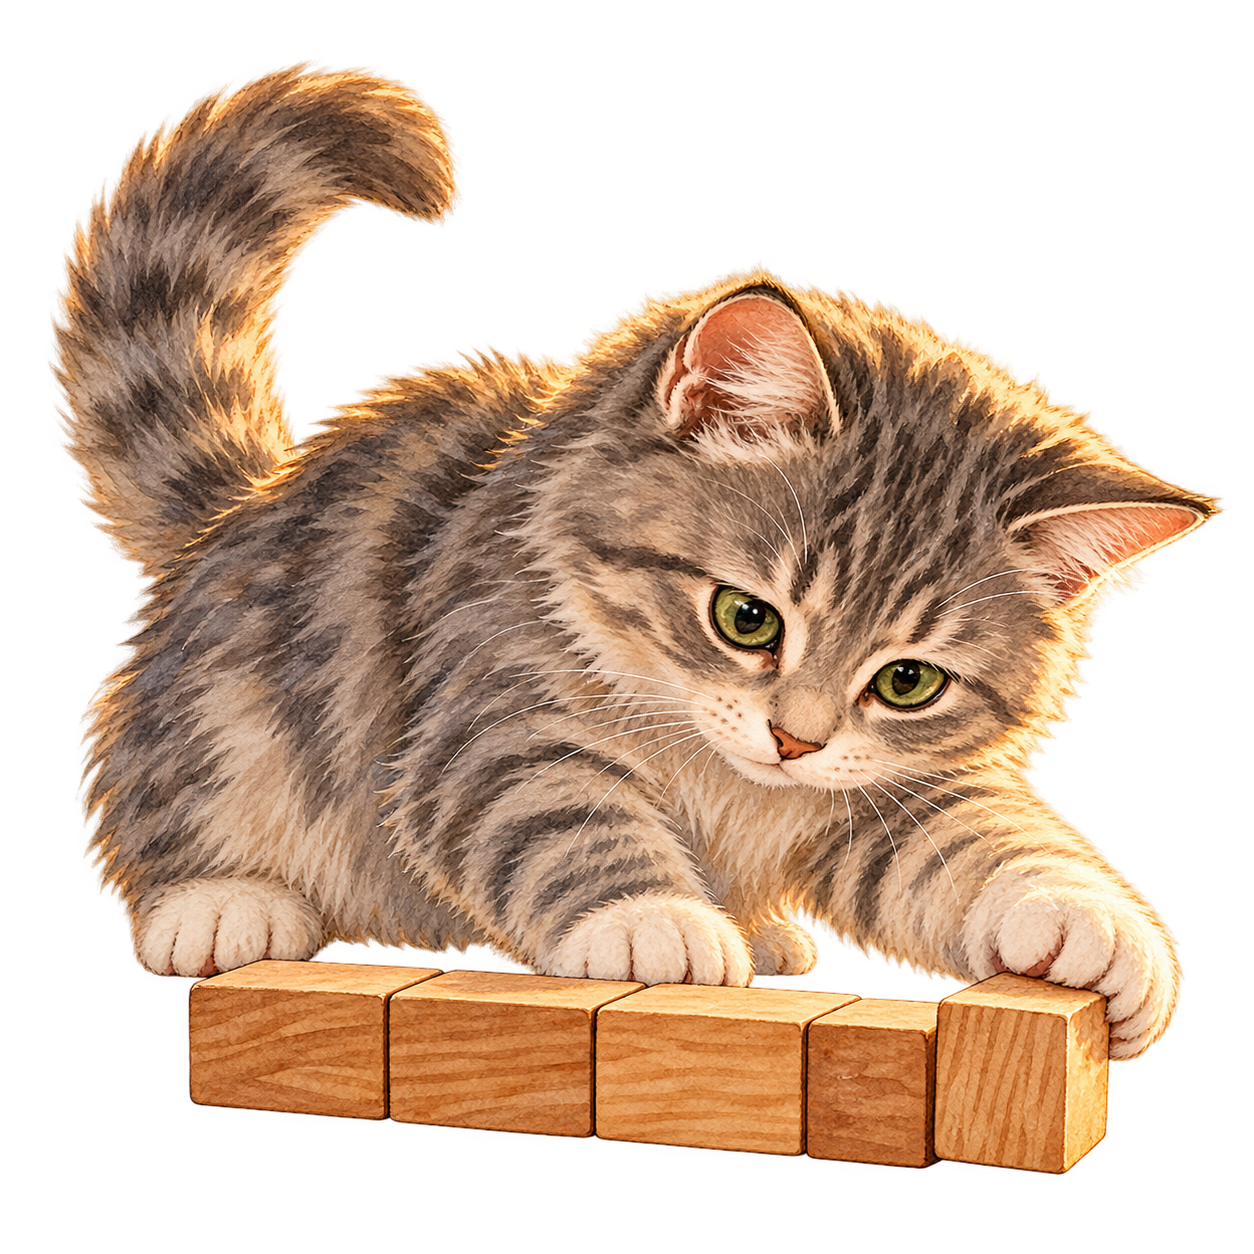
\includegraphics[width=54mm,height=58mm,keepaspectratio]{images/unique/art-20.png}
\label{catflow:20}
\end{wrapfigure}
\textit{Доказательство.} Для неубывающей последовательности супремум \(L\) существует по аксиоме полноты. Выберем любое \(\varepsilon>0\). Число \(L-\varepsilon\) не является верхней гранью, поэтому существует номер \(N\), для которого \(a_N>L-\varepsilon\). При всех \(n\geq N\) по монотонности \(a_n\geq a_N\), а по свойству верхней грани \(a_n\leq L\). Значит, \(L-\varepsilon<a_n\leq L\), то есть \(|a_n-L|<\varepsilon\). Это и означает \(a_n\to L\).

Для невозрастающей и ограниченной снизу последовательности \((a_n)\) последовательность \((-a_n)\) не убывает и ограничена сверху. Уже доказанный случай даёт \(-a_n\to B\), откуда \(a_n\to-B\), поскольку \(|a_n-(-B)|=|-a_n-B|\).\hfill\(\blacksquare\)
\par\WFclear\end{minipage}\end{lrbox}%
\ifdim\dimexpr\ht\CatFlowBox+\dp\CatFlowBox\relax<64mm\dp\CatFlowBox=\dimexpr64mm-\ht\CatFlowBox\relax\fi%
\noindent\usebox{\CatFlowBox}\par\addvspace{5pt}

Условие с \(\varepsilon\) придаёт словам «сколь угодно близко» точный смысл: сначала выбирается любая положительная точность \(\varepsilon\), и только после этого подбирается номер \(N\), начиная с которого \emph{все} члены удовлетворяют \(|a_n-L|<\varepsilon\). Единого заранее фиксированного \(N\) для всех точностей не требуется.

\subsection{Бесконечная сумма}
\begin{definition}
\term{Бесконечный ряд} (infinite series) \(\sum_{n=1}^{\infty}a_n\) \term{сходится} (converges) к числу \(S\), если его частичные суммы \(S_N\) имеют предел \(S\). Число \(S\) называют \term{суммой ряда} (sum of a series). Если такого конечного предела нет, ряд \term{расходится} (diverges).
\end{definition}
\begin{theorem}[Бесконечная геометрическая сумма]\label{thm:legacy-c12-7}
Пусть \(a_{n+1}=q a_n\). При \(|q|<1\)
\[
\sum_{n=1}^{\infty}a_n=\frac{a_1}{1-q}.
\]
Если \(a_1\neq0\), условие \(|q|<1\) также необходимо для сходимости. В частности, при \(q=1\) и при \(q=-1\) такой ряд расходится.
\end{theorem}
\begin{proof}
Сначала покажем \(q^N\to0\) при \(|q|<1\). Случай \(q=0\) непосредственен. Если \(0<r=|q|<1\), то \(r=\frac1{1+h}\) с \(h>0\). Неравенство \((1+h)^N\geq1+Nh\) доказывается индукцией: после умножения \(1+Nh\) на \(1+h\) получаем \(1+(N+1)h+Nh^2\geq1+(N+1)h\). Значит, \(|q^N|=r^N\leq\frac1{1+Nh}\), а эта верхняя граница становится меньше любого \(\varepsilon>0\) при достаточно большом \(N\).

По формуле конечной суммы
\[
\left|S_N-\frac{a_1}{1-q}\right|=\frac{|a_1|\,|q|^N}{|1-q|}\longrightarrow0.
\]
При \(a_1=0\) все суммы уже равны нулю. Если \(a_1\neq0\) и \(|q|\geq1\), то \(|a_n|=|a_1||q|^{n-1}\geq|a_1|\), поэтому \(a_n\) не стремится к нулю. Но из сходимости \(S_N\to S\) обязательно следует \(a_N=S_N-S_{N-1}\to0\): разность ограничена сверху величиной \(|S_N-S|+|S_{N-1}-S|\), и оба слагаемых стремятся к нулю. Получили противоречие.

Наглядно, при \(q=1\) суммы \(S_N=Na_1\) неограниченно растут по модулю. При \(q=-1\) они чередуются: \(S_{2k}=0\), \(S_{2k-1}=a_1\); при \(a_1\neq0\) единого предела нет.
\end{proof}
\begin{example}
\(1+\frac12+\frac14+\cdots=2\). При этом первые \(N\) слагаемых дают \(S_N=2(1-2^{-N})\), а недостающая до \(2\) величина равна \(2^{1-N}\) и стремится к нулю.
\end{example}

\section{Построение числа \(e\)}\label{sec:e-construction}
Положим \(a_n=(1+1/n)^n\).\begin{theorem}[Сходимость последовательности сложных процентов]\label{thm:legacy-c14-1}
Последовательность \(a_n=(1+\frac1n)^n\) строго возрастает, ограничена сверху и имеет предел, лежащий между \(2\) и \(3\).
\end{theorem}
\par\addvspace{5pt}\begin{lrbox}{\CatFlowBox}\begin{minipage}[t]{\linewidth}
\setlength{\parskip}{5pt}\setlength{\columnsep}{4.5mm}\setlength{\intextsep}{0pt}
\begin{wrapfigure}[12]{r}{54mm}

\includegraphics[width=54mm,height=58mm,keepaspectratio]{images/unique/art-28.png}
\label{catflow:28}
\end{wrapfigure}
\textit{Доказательство.} По биному Ньютона \(a_n=\sum_{k=0}^n\frac1{k!}\prod_{j=0}^{k-1}(1-\frac jn)\). Знак \(\sum\) означает сложение слагаемых, \(\prod\) — перемножение множителей; при \(k=0\) произведение принимается равным \(1\). При замене \(n\) на \(n+1\) все множители уже имеющихся слагаемых не уменьшаются и добавляется новое положительное слагаемое. Поэтому \(a_{n+1}>a_n\).
Для \(k\ge2\) имеем \(k!\ge2\cdot3^{k-2}\), поскольку все множители от \(3\) до \(k\) не меньше \(3\). Множители под знаком \(\prod\) лежат в \((0;1]\), поэтому при \(n\ge2\) получаем \(a_n\le2+\frac12\sum_{j=0}^{n-2}(\frac13)^j<2+\frac12\cdot\frac1{1-\frac13}=\frac{11}{4}\); также \(a_1=2<\frac{11}{4}\). По теореме о монотонной ограниченной последовательности предел существует. Он не меньше \(a_2=\frac94>2\) и не больше \(\frac{11}{4}<3\).\hfill\(\blacksquare\)
\par\WFclear\end{minipage}\end{lrbox}%
\ifdim\dimexpr\ht\CatFlowBox+\dp\CatFlowBox\relax<64mm\dp\CatFlowBox=\dimexpr64mm-\ht\CatFlowBox\relax\fi%
\noindent\usebox{\CatFlowBox}\par\addvspace{5pt}

\begin{definition}\term{Число \(e\)} (Euler's number) — предел \(e=\lim_{n\to\infty}(1+\frac1n)^n\), существование которого доказано выше. Приближённо \(e\approx2{,}718281828\).\end{definition}
Предельный результат для начальной суммы \(S\) в описанной модели равен \(Se\); это объясняет появление числа \(e\) при непрерывном накоплении.

\Needspace{7\baselineskip}\section*{Задачи}
\begingroup\setlength{\parskip}{2pt}
\noindent\begin{minipage}[t]{\linewidth}\textbf{37.1.} Найдите сумму бесконечного ряда \(18-6+2-\dfrac23+\cdots\). Объясните, почему геометрическая сумма здесь существует.\par\end{minipage}\par
\par\addvspace{5pt}\begin{lrbox}{\CatFlowBox}\begin{minipage}[t]{\linewidth}
\setlength{\parskip}{5pt}\setlength{\columnsep}{4.5mm}\setlength{\intextsep}{0pt}
\begin{wrapfigure}[12]{l}{54mm}

\includegraphics[width=54mm,height=58mm,keepaspectratio]{images/unique/art-30.png}
\label{catflow:30}
\end{wrapfigure}
\textbf{37.2.} Докажите, что ряд \(a-a+a-a+\cdots\) не имеет суммы в смысле предела частичных сумм, если \(a\neq0\).\par

\textbf{37.3.}\starmark{} Суммируют числа \(64,16,4,1,\ldots\). Найдите бесконечную сумму \(S\), формулу остатка \(R_N=S-S_N\) и наименьшее натуральное \(N\), при котором \(R_N<\dfrac1{10}\).\par

\textbf{37.4.} Для множества \((-2;5]\) найди супремум, инфимум, наибольший и наименьший элементы, если они существуют.\par

\textbf{37.5.} Найди точные грани множества \(A=\{1+\dfrac1n:n\in\mathbb N\}\). Принадлежат ли они \(A\)? Обоснуй ответ.\par

\textbf{37.6.} Для \(A=\{-3,2,7\}\) перечисли все нижние и верхние грани. Укажи точные грани.\par

\textbf{37.7.} Пусть непустое \(A\subseteq\mathbb R\) ограничено снизу, \(c\in\mathbb R\). Докажи \(\inf\{c+a:a\in A\}=c+\inf A\).\par
\par\WFclear\end{minipage}\end{lrbox}%
\ifdim\dimexpr\ht\CatFlowBox+\dp\CatFlowBox\relax<64mm\dp\CatFlowBox=\dimexpr64mm-\ht\CatFlowBox\relax\fi%
\noindent\usebox{\CatFlowBox}\par\addvspace{5pt}

\noindent\begin{minipage}[t]{\linewidth}\textbf{37.8.} Докажи по определению, что \(1/n\to0\). Для \(\varepsilon=0{,}01\) укажи подходящий номер \(N\).\par\end{minipage}\par
\noindent\begin{minipage}[t]{\linewidth}\textbf{37.9.} Докажи, что \(a_n=2-1/n\) возрастает, ограничена и сходится к \(2\).\par\end{minipage}\par
\noindent\begin{minipage}[t]{\linewidth}\textbf{37.10.} Сходится ли \(a_n=(-1)^n\)? Обоснуй ответ.\par\end{minipage}\par
\noindent\begin{minipage}[t]{\linewidth}\textbf{37.11.} Найди предел \(\dfrac{3n+1}{n+2}\) и оцени ошибку через \(n\).\par\end{minipage}\par
\noindent\begin{minipage}[t]{\linewidth}\textbf{37.12.}\starmark{} Докажи, что сходящаяся действительная последовательность ограничена.\par\end{minipage}\par
\noindent\begin{minipage}[t]{\linewidth}\textbf{37.13.}\starmark{} Докажи единственность предела последовательности.\par\end{minipage}\par
\noindent\begin{minipage}[t]{\linewidth}\textbf{37.14.}\starmark{} Пусть \(a_n\le b_n\le c_n\) и \(a_n,c_n\to L\). Докажи \(b_n\to L\).\par\end{minipage}\par
\endgroup
